\chapter{Results and Discussion}
\label{ch:results}

All numbers in this chapter are generated from the CSV files the evaluation
scripts write (\code{results/}), and all timings were measured on a 2-core
cloud virtual machine with the CPU otherwise idle. Absolute timings on other
hardware differ; the comparisons between suites do not.

\section{Cryptographic cost}

\subsection{Primitives}

\begin{table}[h]
\centering
\caption{Primitive operations (ms)}
\label{tab:prim}
\small
\begin{adjustbox}{max width=\linewidth}
\begin{tabular}{lrrrrrr}
\toprule
Suite & KEM keygen & encaps & decaps & sign & sign p99 & verify \\
\midrule
Classical & 0.024 & 0.12 & 0.091 & 0.031 & 0.072 & 0.12 \\
L1 (KEM in kyber-py) & 1.80 & 2.70 & 3.63 & 1.27 & 3.32 & 0.16 \\
L3 & 0.14 & 0.052 & 0.041 & 1.30 & 4.60 & 0.23 \\
DECK & 0.23 & 0.067 & 0.052 & 1.28 & 4.38 & 0.23 \\
L5 & 0.20 & 0.067 & 0.052 & 1.48 & 5.19 & 0.42 \\
\bottomrule
\end{tabular}
\end{adjustbox}
\par\smallskip{\footnotesize Mean of 200 runs after warm-up, in ms. All operations use OpenSSL through the \texttt{cryptography} library, except L1's ML-KEM-512, which that library does not expose; it comes from \texttt{kyber-py} (pure Python).}

\end{table}

Table~\ref{tab:prim} gives two findings. First, \textbf{signing is the only
expensive post-quantum operation, and its variance is intrinsic}: ML-DSA's
rejection sampling repeats until a candidate passes, so the 99th percentile
is several times the mean in both backends, while verification is
deterministic and fast. Second, \textbf{the implementation matters more than
the algorithm}: the same ML-DSA-65 signs in \V{deck-sign-native}\,ms natively
and \V{deck-sign-pure}\,ms in pure Python, a factor of about \V{sign-speedup}.
Our Review~1 conclusion, that signing might not fit the 100\,ms budget, was a
property of the pure-Python library, not of ML-DSA.

\subsection{Handshake size and compute}

\begin{table}[h]
\centering
\caption{Key, signature, certificate and handshake sizes (bytes), with and without certificate caching}
\label{tab:sizes}
\scriptsize
\setlength{\tabcolsep}{3.2pt}
\begin{adjustbox}{max width=\linewidth}
\begin{tabular}{lllrrrrrrrrr}
\toprule
Suite & KEM & Signature & pk$_\text{KEM}$ & sig & cert & bytes & frames & air (ms) & cached & frames & saving \\
\midrule
Classical & ECDH-P256 & ECDSA-P256 & 65 & 70 & 229 & 1{,}043 & 4 & 2.05 & 691 & 4 & 33.7\,\% \\
L1 & ML-KEM-512 & ML-DSA-44 & 800 & 2{,}420 & 3{,}826 & 14{,}373 & 13 & 21.3 & 6{,}825 & 8 & 52.5\,\% \\
L3 & ML-KEM-768 & ML-DSA-65 & 1{,}184 & 3{,}309 & 5{,}355 & 19{,}913 & 17 & 29.4 & 9{,}307 & 10 & 53.3\,\% \\
DECK & ML-KEM-1024 & ML-DSA-65 & 1{,}568 & 3{,}309 & 5{,}355 & 20{,}779 & 17 & 30.5 & 10{,}173 & 10 & 51.0\,\% \\
L5 & ML-KEM-1024 & ML-DSA-87 & 1{,}568 & 4{,}627 & 7{,}313 & 27{,}329 & 22 & 40.1 & 12{,}807 & 12 & 53.1\,\% \\
\bottomrule
\end{tabular}
\end{adjustbox}

\end{table}

\begin{figure}[h]
\centering
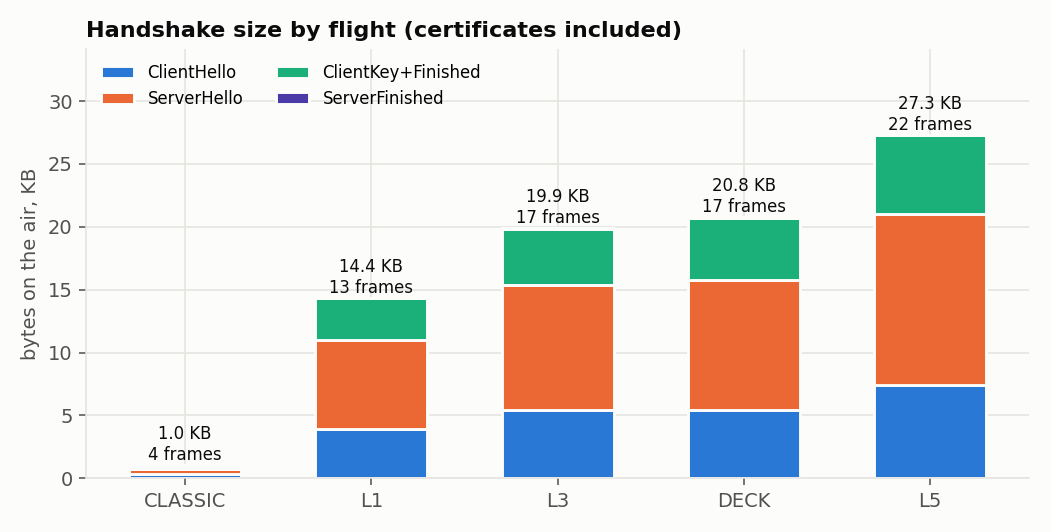
\includegraphics[width=0.9\textwidth]{fig2_handshake_size.png}
\caption{Handshake bytes by flight. The ServerHello carries the server's certificate, the ephemeral ML-KEM key and a signature.}
\label{fig:size}
\end{figure}

\begin{table}[h]
\centering
\caption{Compute time of one full handshake, both sides (ms)}
\label{tab:hstime}
\begin{adjustbox}{max width=\linewidth}
\begin{tabular}{lrr}
\toprule
Suite & mean & p95 \\
\midrule
Classical & 1.16 & 1.29 \\
L1 & 11.6 & 12.6 \\
L3 & 4.77 & 7.85 \\
DECK & 4.77 & 7.22 \\
L5 & 5.68 & 8.12 \\
\bottomrule
\end{tabular}
\end{adjustbox}
\par\smallskip{\footnotesize Compute time of one complete mutual handshake, both sides together, in ms (no network).}

\end{table}

A post-quantum handshake is \V{pq-size-ratio-lo}--\V{pq-size-ratio-hi} times
the size of the classical one (Table~\ref{tab:sizes},
Figure~\ref{fig:size}): \V{deck-hs-bytes} bytes in \V{deck-hs-frames} frames
for DECK against \V{classic-hs-bytes} bytes in \V{classic-hs-frames} frames,
or \V{deck-hs-air}\,ms of airtime against \V{classic-hs-air}\,ms. Certificates
are the largest single item, \V{deck-cert} bytes each. The Review~1 figure of
6,494 bytes left the certificates out.

Computation is small by comparison (Table~\ref{tab:hstime},
Figure~\ref{fig:compute}): about \V{deck-hs-ms}\,ms for a complete DECK
handshake natively against \V{classic-hs-ms}\,ms classically, but
\V{deck-hs-ms-pure}\,ms with the pure-Python library. With a native
implementation, \textbf{the cost of post-quantum V2X is bytes, not CPU time}.

\begin{figure}[h]
\centering
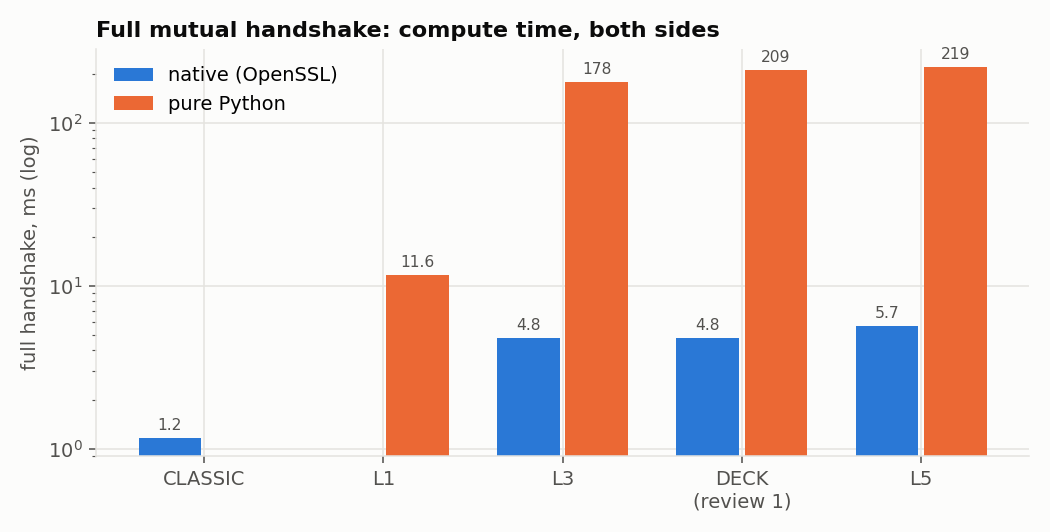
\includegraphics[width=0.85\textwidth]{fig1_handshake_compute.png}
\caption{Full handshake compute time, native and pure-Python backends (log scale).}
\label{fig:compute}
\end{figure}

\subsection{Per-beacon budget}

\begin{table}[h]
\centering
\caption{Per-beacon cost, p99 crypto plus airtime (ms)}
\label{tab:beacon}
\small
\begin{adjustbox}{max width=\linewidth}
\begin{tabular}{lrr}
\toprule
Suite & AEAD in a session & signed broadcast \\
\midrule
Classical & 0.40 (135 B) & 0.88 (234 B, 1 fr.) \\
L1 & 0.44 (135 B) & 5.55 (2{,}583 B, 2 fr.) \\
L3 & 0.41 (135 B) & 9.87 (3{,}472 B, 3 fr.) \\
DECK & 0.41 (135 B) & 9.51 (3{,}472 B, 3 fr.) \\
L5 & 0.47 (135 B) & 12.6 (4{,}790 B, 4 fr.) \\
\bottomrule
\end{tabular}
\end{adjustbox}
\par\smallskip{\footnotesize p99 of cryptographic processing plus 802.11p airtime per beacon, in ms, against the 100 ms beacon interval.}

\end{table}

The base paper folds the one-off handshake into its per-message latency.
Separated (Table~\ref{tab:beacon}, Figure~\ref{fig:beacon}), the per-beacon
cost inside a session is the same for every suite: a
\V{deck-beacon-aead-bytes}-byte AES-GCM record costing
\V{deck-beacon-aead}\,ms against a 100\,ms interval. Signing every beacon, as
IEEE~1609.2 does today, also fits natively (\V{deck-beacon-signed}\,ms for
DECK) but costs \V{deck-beacon-signed-bytes} bytes, \V{deck-beacon-signed-frames}
frames per beacon, and misses the deadline with the pure-Python library.

\begin{figure}[h]
\centering
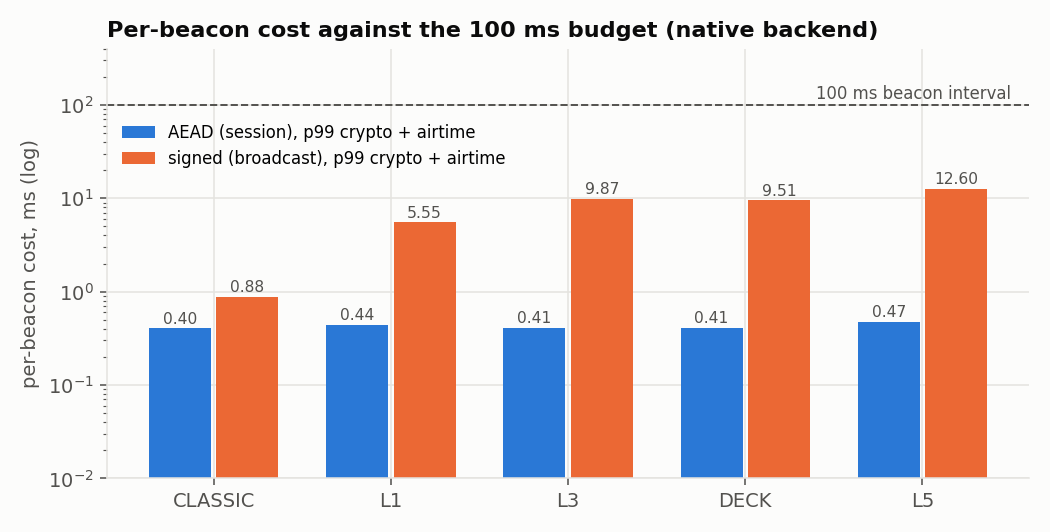
\includegraphics[width=0.85\textwidth]{fig3_beacon_budget.png}
\caption{Per-beacon cost against the 100\,ms beacon interval.}
\label{fig:beacon}
\end{figure}

\section{Distributed system}

One run of the demonstration scenario (19 processes over TCP on one machine)
established \V{net-handshakes} secure sessions (\V{net-hs-min}--\V{net-hs-max}
bytes each, depending on whether certificates travelled as references) and
rejected \V{net-rejected} handshakes from the revoked vehicle. Alerts reached
vehicles a median \V{net-alert-ms}\,ms after a critical event was reported,
while the event reached the ledger after a median \V{net-ledger-ms}\,ms: the
MEC sends the alert before it submits the event, so \textbf{the safety path
never waits for consensus}. The Byzantine node (wrong results) was demoted at
the first regroup and a candidate promoted; when the leader crashed, a view
change installed the next leader and later events committed; after the TA
revoked a vehicle, its session was closed and its reconnection rejected. All
eight ledger copies were consistent (the crashed leader's copy is a prefix
of the others) and verified from genesis.

\section{ns-3: 802.11p with mobility}

\subsection{Handshake success and latency}

\begin{table}[h]
\centering
\caption{Handshakes completed (\%) by vehicle density}
\label{tab:ns3success}
\small
\begin{adjustbox}{max width=\linewidth}
\begin{tabular}{lrrrrrr}
\toprule
Vehicles (/km$^2$) & Classical & L1 & L3 & DECK & L5 & DECK + cache \\
\midrule
50 (22) & 100 & 100 & 99 & 100 & 99 & 100 \\
100 (44) & 100 & 97 & 70 & 74 & 56 & 98 \\
150 (67) & 100 & 54 & 40 & 38 & 32 & 80 \\
200 (89) & 100 & 39 & 27 & 27 & 22 & 57 \\
\bottomrule
\end{tabular}
\end{adjustbox}
\par\smallskip{\footnotesize Handshakes completed, \%. Mean of 3 seeds; 1.5\,km $\times$ 1.5\,km Manhattan grid, 9 RSUs, IEEE 802.11p at 6\,Mb/s.}

\end{table}

\begin{table}[h]
\centering
\caption{Median handshake completion time (ms)}
\label{tab:ns3p50}
\small
\begin{adjustbox}{max width=\linewidth}
\begin{tabular}{lrrrrrr}
\toprule
Vehicles (/km$^2$) & Classical & L1 & L3 & DECK & L5 & DECK + cache \\
\midrule
50 (22) & 7 & 73 & 88 & 90 & 139 & 54 \\
100 (44) & 8 & 109 & 288 & 285 & 482 & 73 \\
150 (67) & 10 & 575 & 651 & 636 & 750 & 197 \\
200 (89) & 12 & 763 & 760 & 795 & 844 & 417 \\
\bottomrule
\end{tabular}
\end{adjustbox}
\par\smallskip{\footnotesize Median handshake completion time, ms. Mean of 3 seeds; 1.5\,km $\times$ 1.5\,km Manhattan grid, 9 RSUs, IEEE 802.11p at 6\,Mb/s.}

\end{table}

\begin{figure}[h]
\centering
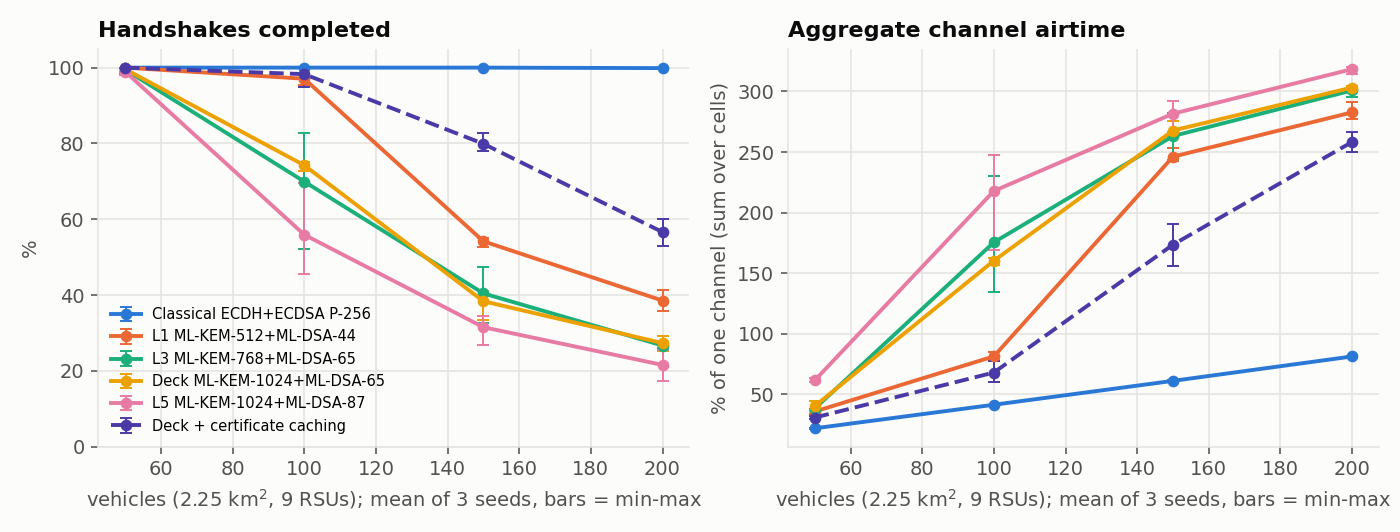
\includegraphics[width=\textwidth]{fig8_ns3_success_airtime.png}
\caption{Handshakes completed and aggregate channel airtime against density (mean of \V{ns3-seeds} seeds, bars show min--max).}
\label{fig:ns3success}
\end{figure}

\begin{figure}[h]
\centering
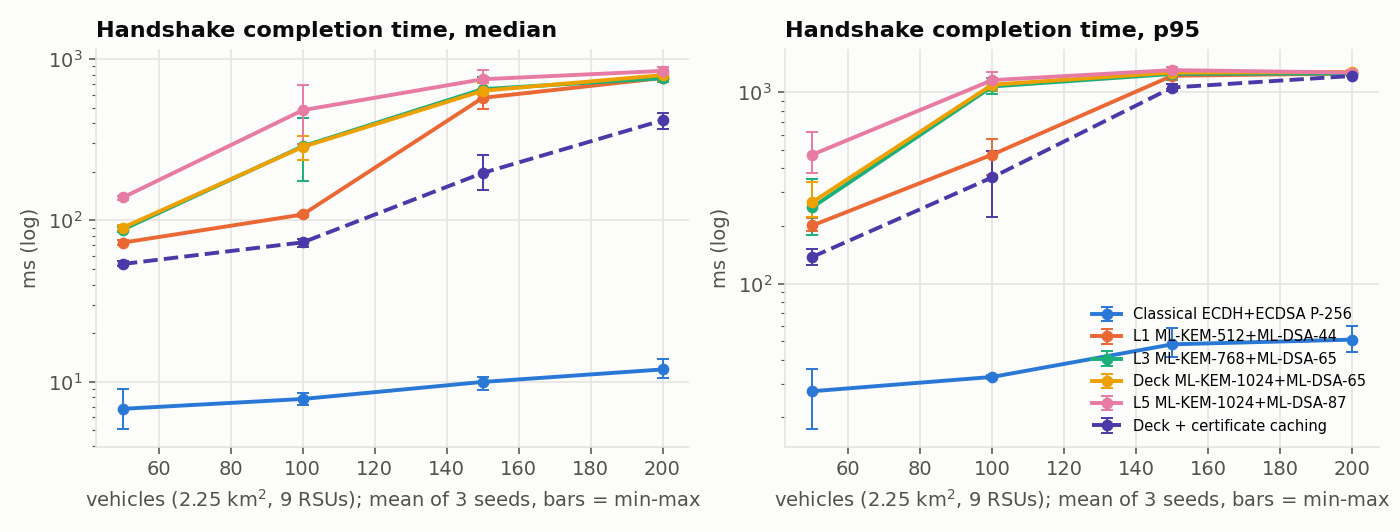
\includegraphics[width=\textwidth]{fig7_ns3_handshake_latency.png}
\caption{Handshake completion time, median and 95th percentile (log scale).}
\label{fig:ns3lat}
\end{figure}

Tables~\ref{tab:ns3success} and~\ref{tab:ns3p50} and
Figures~\ref{fig:ns3success}--\ref{fig:ns3lat} give the central result.
\textbf{The classical handshake completes \V{ns3-success-classic-200}\,\% of the
time even at 200 vehicles. Every post-quantum suite degrades with density},
roughly in order of handshake size: L1 (\V{l1-hs-kb}\,KB) holds up longest
and L5 (\V{l5-hs-kb}\,KB) fails first, while L3 and DECK, which differ by
less than 1\,KB, are within seed-to-seed variation of each other. At 100 vehicles (44 per
km$^2$) DECK completes \V{ns3-success-deck-100}\,\% of handshakes with a
median of \V{ns3-p50-deck-100}\,ms, against \V{ns3-p50-classic-100}\,ms
classically; at 200 vehicles it completes \V{ns3-success-deck-200}\,\%.
The cause is airtime: handshake fragments push the shared channel into
saturation, and losses then trigger retransmissions that add more load.

\subsection{Other measures}

\begin{table}[h]
\centering
\caption{Other measures at \V{ns3-mid} vehicles}
\label{tab:ns3mid}
\small
\begin{adjustbox}{max width=\linewidth}
\begin{tabular}{lrrr}
\toprule
Measure & Classical & DECK & DECK + cache \\
\midrule
Beacon slots with a session (\%) & 99.9 & 83.3 & 97.4 \\
Aggregate airtime (\% of one channel) & 41 & 160 & 68 \\
Handshake time, p95 (ms) & 33 & 1{,}094 & 359 \\
Event $\rightarrow$ alert at the reporter, median (ms) & 5.4 & 7.6 & 5.6 \\
Ledger commit after the event, median (ms) & 11.6 & 24.6 & 24.0 \\
Sessions lost (link timeout) & 0.0 & 3.0 & 1.7 \\
\bottomrule
\end{tabular}
\end{adjustbox}
\par\smallskip{\footnotesize 100 vehicles, mean of 3 seeds.}

\end{table}

\begin{figure}[h]
\centering
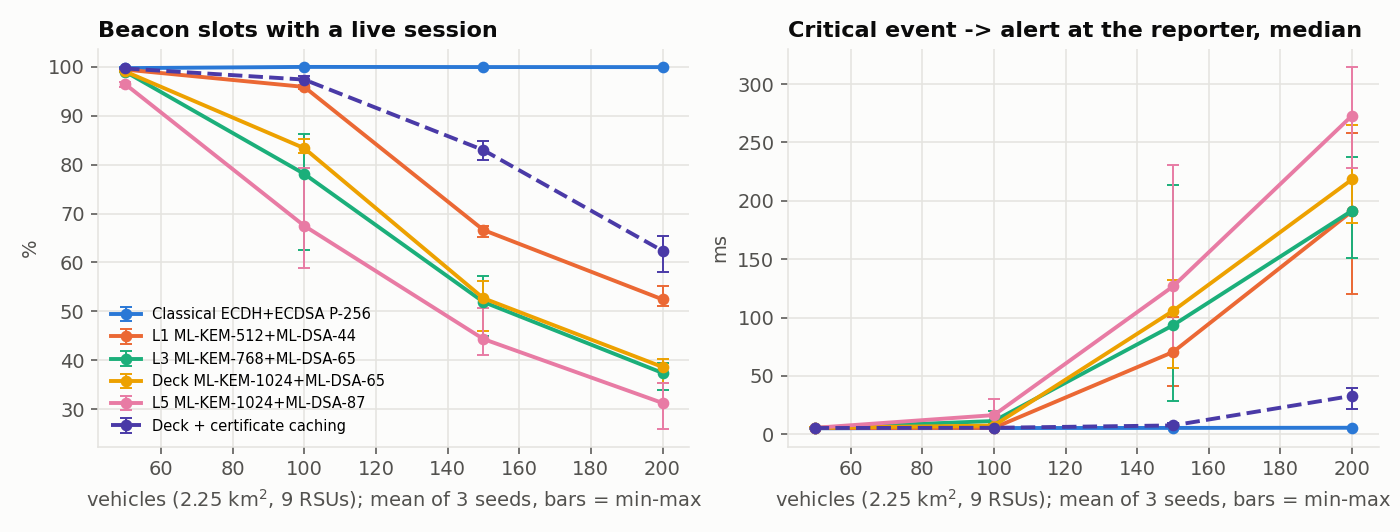
\includegraphics[width=\textwidth]{fig9_ns3_coverage_alert.png}
\caption{Beacon slots with a live session, and the time from a critical event to the alert at the reporting vehicle.}
\label{fig:ns3cov}
\end{figure}

Table~\ref{tab:ns3mid} and Figure~\ref{fig:ns3cov} show the consequence for
safety messaging. A vehicle without a session cannot send authenticated
beacons, so the fraction of beacon slots covered by a session falls with the
handshake success rate. Up to 100 vehicles alerts stay below 20\,ms for every
suite, from \V{ns3-alert-classic-100}\,ms (classical) to
\V{ns3-alert-l5-100}\,ms (L5) median. Beyond that, a saturated channel
delays them too: at 200 vehicles the median is \V{ns3-alert-deck-200}\,ms for
DECK and \V{ns3-alert-deck-cache-200}\,ms with caching, against
\V{ns3-alert-classic-200}\,ms classically.

\subsection{Certificate caching}

\begin{figure}[h]
\centering
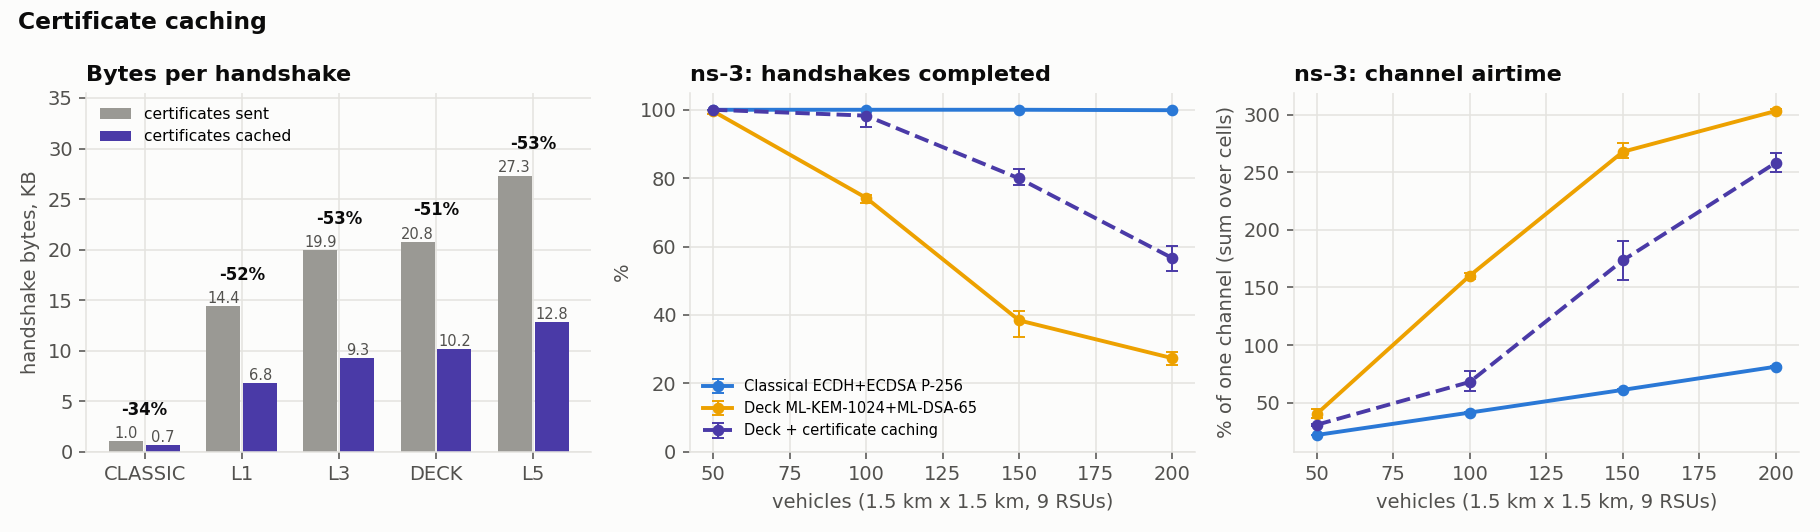
\includegraphics[width=\textwidth]{fig11_cert_cache.png}
\caption{Certificate caching: bytes per handshake for every suite, and its effect on DECK in ns-3.}
\label{fig:cache}
\end{figure}

Caching removes \V{pq-cache-lo}--\V{pq-cache-hi}\,\% of every
post-quantum handshake (Table~\ref{tab:sizes}). In ns-3
(Figure~\ref{fig:cache}), with RSU certificates pre-distributed and vehicle
certificates resolved from the MEC directory, DECK completes
\V{ns3-success-deck-cache-100}\,\% of handshakes at 100 vehicles instead of
\V{ns3-success-deck-100}\,\%, and \V{ns3-success-deck-cache-200}\,\% at 200
instead of \V{ns3-success-deck-200}\,\%; aggregate airtime at 100 vehicles
falls from \V{ns3-airtime-deck-100}\,\% to \V{ns3-airtime-deck-cache-100}\,\%.
Caching does not close the gap to the classical suite: a cached DECK
handshake is still \V{deck-cached-bytes} bytes, about ten times a classical
one, because the ephemeral ML-KEM key, the ciphertext and two ML-DSA
signatures cannot be cached.

\subsection{Variants and mitigations}

\begin{table}[h]
\centering
\caption{Single-seed variants at \V{ns3-mid} vehicles}
\label{tab:variants}
\small
\begin{adjustbox}{max width=\linewidth}
\begin{tabular}{lrrrrr}
\toprule
Scenario (seed 1) & completed \% & p50 ms & coverage \% & alert ms & airtime \% \\
\midrule
DECK, EDCA + backoff (baseline) & 75 & 283 & 82.3 & 7.2 & 157 \\
DECK, neither & 7 & 921 & 40.1 & 432.6 & 339 \\
DECK, EDCA only & 11 & 926 & 44.3 & 382.3 & 330 \\
DECK, backoff only & 77 & 291 & 84.6 & 8.9 & 174 \\
\midrule
DECK + cache (directory) & 100 & 68 & 97.9 & 5.5 & 66 \\
DECK + cache (all warm) & 97 & 66 & 98.5 & 6.0 & 66 \\
L3 + cache (directory) & 100 & 76 & 97.1 & 5.9 & 71 \\
\midrule
DECK, signed beacons & 23 & 704 & 45.9 & 232.9 & 342 \\
Classical, signed beacons & 100 & 9 & 99.9 & 5.4 & 54 \\
\bottomrule
\end{tabular}
\end{adjustbox}
\par\smallskip{\footnotesize Single-seed variants at 100 vehicles. Coverage: beacon slots with a live session. Alert: event $\rightarrow$ alert at the reporter, median. Airtime: summed over all cells.}

\end{table}

\begin{figure}[h]
\centering
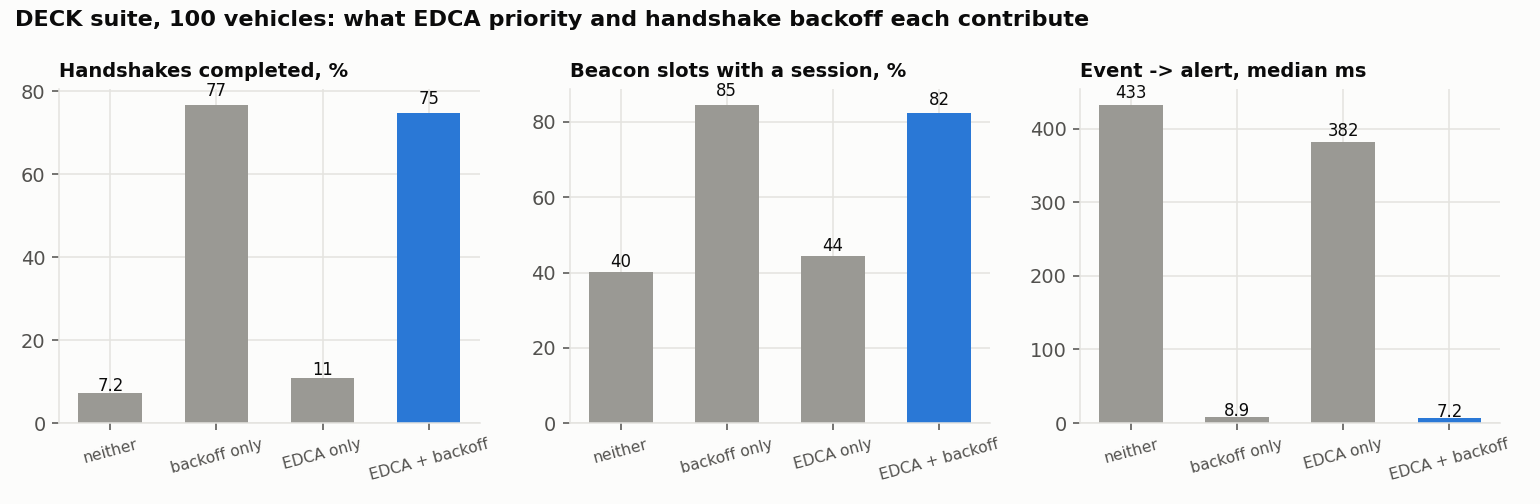
\includegraphics[width=\textwidth]{fig10_ns3_ablation.png}
\caption{Ablation: what EDCA priority and handshake backoff each contribute (DECK, \V{ns3-mid} vehicles).}
\label{fig:ablation}
\end{figure}

Table~\ref{tab:variants} and Figure~\ref{fig:ablation} show four further
results.
\begin{enumerate}
\item \textbf{Exponential backoff prevents congestion collapse.} Without it,
failed handshakes are retried immediately: DECK completes only
\V{var-deck-neither-success}\,\% of handshakes (\V{var-deck-edca-only-success}\,\%
with EDCA alone), and alerts take a median \V{var-deck-neither-alert}\,ms
because they queue behind handshake fragments. With backoff alone DECK
completes \V{var-deck-backoff-only-success}\,\% and alerts take
\V{var-deck-backoff-only-alert}\,ms.
\item \textbf{EDCA priority adds little once backoff is on, at this density.}
With both measures DECK completes \V{var-deck-edca-backoff-baseline-success}\,\%
of handshakes and the alert median is \V{var-deck-edca-backoff-baseline-alert}\,ms,
within single-seed noise of backoff alone. Its value is as a safeguard: it
keeps safety traffic ahead of handshake fragments whenever the queue builds up.
\item \textbf{Signed beacons do not scale with post-quantum signatures.}
Signing every beacon (\V{deck-beacon-signed-frames} frames each) leaves
\V{var-deck-signed-beacons-coverage}\,\% of beacon slots covered, against
\V{var-classical-signed-beacons-coverage}\,\% classically. Session-based AEAD
beacons are the design that scales.
\item \textbf{The implementation still matters in the network.} With
processing times from the pure-Python library, DECK completes
\V{var-deck-pure-python-timings-success}\,\% of handshakes (native:
\V{var-deck-edca-backoff-baseline-success}\,\%) and its median handshake takes
\V{var-deck-pure-python-timings-p50}\,ms instead of
\V{var-deck-edca-backoff-baseline-p50}\,ms.
\end{enumerate}

\section{Consensus}

\begin{table}[h]
\centering
\caption{AGS-PBFT against PBFT}
\label{tab:cons}
\small
\setlength{\tabcolsep}{4pt}
\begin{adjustbox}{max width=\linewidth}
\begin{tabular}{rrrrrrrr}
\toprule
Nodes & $|CN|$ & msgs/req AGS / PBFT & fewer msgs \% & fewer bytes \% & no shadow \% & latency \% & less CPU \% \\
\midrule
8 & 4 & 35 / 128 & 73 & 8 & 41 & +49 & 18 \\
12 & 4 & 47 / 288 & 84 & 23 & 64 & +46 & 25 \\
16 & 7 & 89 / 512 & 83 & 25 & 57 & +41 & 18 \\
20 & 10 & 149 / 800 & 81 & 25 & 53 & +43 & 23 \\
24 & 10 & 161 / 1{,}152 & 86 & 30 & 63 & +58 & 24 \\
\bottomrule
\end{tabular}
\end{adjustbox}
\par\smallskip{\footnotesize Real ML-DSA-65 signatures, 1\,ms links, 20 requests at light load. Percentages are AGS-PBFT relative to PBFT; latency is the median commit latency.}

\end{table}

\begin{figure}[h]
\centering
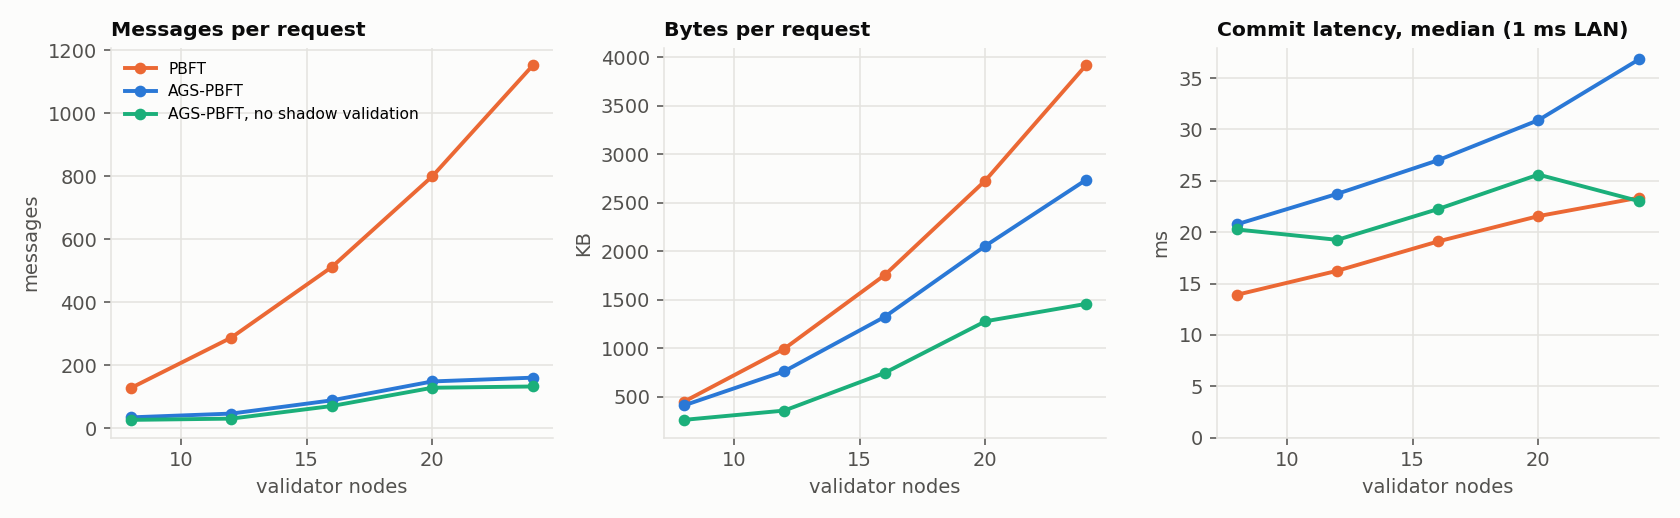
\includegraphics[width=0.9\textwidth]{fig4_consensus_scaling.png}
\caption{Messages, bytes and latency per request against network size.}
\label{fig:cons}
\end{figure}

\textbf{The paper's message saving is real} (Table~\ref{tab:cons},
Figure~\ref{fig:cons}): AGS-PBFT sends \V{cons-msg-8}\,\% fewer messages
than PBFT at 8 nodes and \V{cons-msg-rest-lo}--\V{cons-msg-hi}\,\% fewer at
12--24 nodes, and at light load it uses \V{cons-cpu-lo}--\V{cons-cpu-hi}\,\%
less CPU, because only the $3f+1$ consensus set votes. \textbf{Bytes fall much less}
(\V{cons-byte-lo}--\V{cons-byte-hi}\,\%): every block carries a commit
certificate of $2f+1$ ML-DSA signatures, and with shadow validation (D7) the
candidates' responses as well. Without shadow validation the byte saving is
\V{cons-noshadow-byte-lo}--\V{cons-noshadow-byte-hi}\,\%, but candidates can
then never earn promotion. \textbf{AGS-PBFT is not faster}: replacing PBFT's
parallel all-to-all commit with responses to the leader and a certified block
adds a sequential hop through one node, so commit latency rises by
\V{cons-lat-lo}--\V{cons-lat-hi}\,\%, and under a burst of 60 requests on 16
nodes AGS-PBFT commits \V{tps-ags} requests per second against \V{tps-pbft}
for PBFT, and in that run it used \V{burst-cpu-more}\,\% \emph{more} CPU in
total (\V{burst-cpu-ags}\,s against \V{burst-cpu-pbft}\,s); we have not yet
isolated why the light-load saving reverses under a burst. The paper reports
only the message count.

\begin{table}[h]
\centering
\caption{Fault tolerance}
\label{tab:fault}
\small
\begin{adjustbox}{max width=\linewidth}
\begin{tabular}{lrrrrrr}
\toprule
Byzantine nodes & 0 & 1 & 2 & 3 & 4 & 5 \\
\midrule
Requests committed (\%) & 100 & 100 & 100 & 0 & 0 & 0 \\
Safety held & yes & yes & yes & yes & yes & yes \\
\bottomrule
\end{tabular}
\end{adjustbox}
\par\smallskip{\footnotesize Consensus set 7, f = 2, colluding wrong results, regrouping off.}

\end{table}

\begin{table}[h]
\centering
\caption{Recovery after a leader crash}
\label{tab:vc}
\small
\begin{adjustbox}{max width=\linewidth}
\begin{tabular}{lrr}
\toprule
View-change timeout & AGS-PBFT & PBFT \\
\midrule
0.5 s & 1.21 s & 1.19 s \\
1.0 s & 2.22 s & 2.17 s \\
2.0 s & 4.72 s & 4.68 s \\
\bottomrule
\end{tabular}
\end{adjustbox}
\par\smallskip{\footnotesize Time from the leader's crash to the first commit in the new view (8 nodes).}

\end{table}

Table~\ref{tab:fault} shows PBFT's liveness bound: up to $f$ colluding
Byzantine nodes nothing changes, and beyond $f$ the honest nodes can no longer
form a $2f+1$ quorum, so progress stops. No false result was committed in any
run, but this experiment keeps the leader honest, and an honest leader never
certifies a result that differs from its own. With 5 colluders in a set of 7
the colluders could form a quorum of 5 on their own, so a Byzantine
\emph{leader} beyond $f$ could commit a false result, exactly as PBFT theory
predicts. Recovery after a leader crash (Table~\ref{tab:vc}) takes about
2.2--2.4 times the view-change timeout, because the client's retransmission
timeout and the backups' view-change timeout run one after the other.

\begin{figure}[h]
\centering
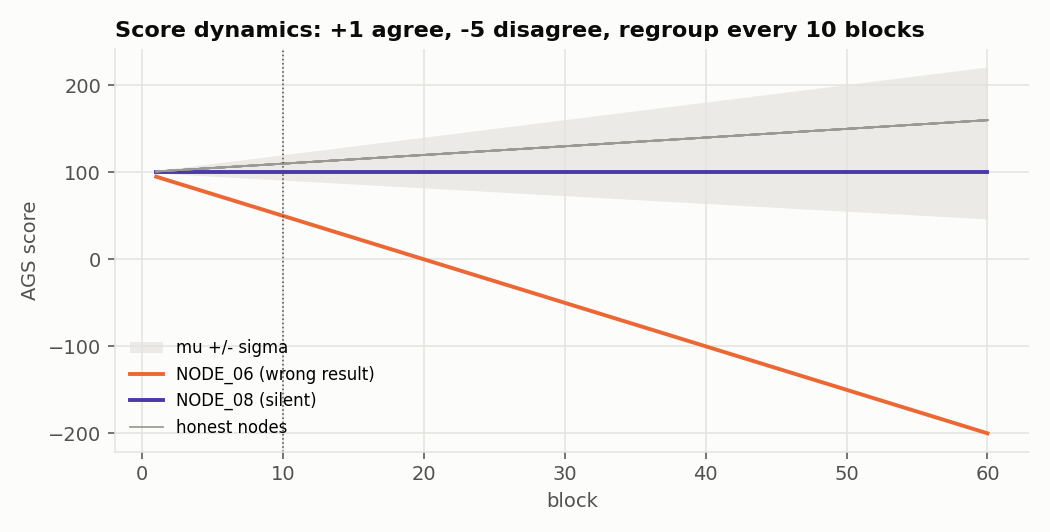
\includegraphics[width=0.9\textwidth]{fig5_score_dynamics.png}
\caption{Score dynamics with one wrong-result node and one silent node (16 nodes, regroup every 10 blocks).}
\label{fig:scores}
\end{figure}

Figure~\ref{fig:scores} shows a weakness of the paper's $\mu \pm \sigma$
rule. The wrong-result node loses 5 points per block and is demoted at the
first regroup. The silent node keeps its score of 100 while honest nodes
climb, but the wrong-result node's extreme score inflates $\sigma$ so much
that $\mu - \sigma$ stays below 100, and the silent node is never demoted.
Without the outlier it is demoted (a regression test checks both cases). A
robust statistic, such as the median and the median absolute deviation, would
not be distorted by one extreme node.

\section{Security}

\begin{table}[h]
\centering
\caption{Attacks run against the implementation}
\label{tab:attacks}
\scriptsize
\begin{adjustbox}{max width=\linewidth}
\begin{tabular}{p{5.4cm}cp{7.2cm}}
\toprule
Attack & Rejected & Mechanism \\
\midrule
record tampering (1 bit flipped) & yes & AES-256-GCM tag check fails \\
record replay & yes & counter already seen in the 64-record window \\
GCM nonce reuse with Finished & yes & data counters start at 1; 0 is Finished only \\
ClientHello replay & yes & nonce already in the server's replay cache \\
stale ClientHello (timestamp -300 s) & yes & outside the 30 s freshness window \\
client impersonation with stolen certificate & yes & client signature over the transcript fails (deck design had no client signature) \\
RSU impersonation with stolen certificate & yes & server signature over transcript + pk\_kem fails \\
certificate from a rogue TA & yes & certificate signature does not verify under pk\_TA \\
revoked credential & yes & certificate serial on the signed CRL \\
cache: claim another vehicle's cached certificate & yes & client signature checked with the referenced certificate's key \\
cache: revoked certificate still in the cache & yes & cached certificates are re-verified against the current CRL \\
vehicle posing as an RSU & yes & role is bound into the certificate \\
MITM substitutes the ephemeral ML-KEM key & yes & server signature covers pk\_kem \\
MITM substitutes the KEM ciphertext & yes & client signature covers c \\
downgrade to classical suite & yes & suite must match and is inside both signatures \\
tampered Finished & yes & key confirmation under transcript-bound keys fails \\
forward secrecy: ephemeral key retained & yes & ephemeral ML-KEM key per session, erased after decapsulation \\
consensus vote from a non-member & yes & sender has no certificate in the directory \\
consensus vote spoofing another member & yes & ML-DSA signature does not verify \\
tampered block (result changed) & yes & leader signature and commit certificate \\
ledger history rewrite & yes & Pr\_B\_Hash link broken \\
\bottomrule
\end{tabular}
\end{adjustbox}

\end{table}

All \V{attacks-total} attacks in Table~\ref{tab:attacks} were rejected. Client
impersonation with a copied certificate would succeed against the Review~1
design, which had no client signature (F2).

\section{Answers to the research questions}

\begin{enumerate}
\item \textbf{Can the framework be implemented with the standardised
algorithms?} Yes, after the corrections D1--D5 and F1--F7 and the design
decisions D6--D9; the result runs as a distributed system and withstands the
tested attacks.
\item \textbf{Does post-quantum protection fit the 100\,ms budget?} Per
message, yes, at every security level: \V{deck-beacon-aead}\,ms per beacon
inside a session, or \V{deck-beacon-signed}\,ms for a natively signed beacon.
A full handshake costs about \V{deck-hs-ms}\,ms of computation natively.
\item \textbf{How does the channel behave as density grows?} The handshake
is the problem: at 100 vehicles DECK completes \V{ns3-success-deck-100}\,\% of
handshakes against \V{ns3-success-classic-100}\,\% classically. Certificate
caching and exponential backoff recover much of the loss; a smaller KEM (L3
instead of DECK) costs nothing in security, since DECK's strength is set by
its category-3 signature.
\item \textbf{Does AGS-PBFT beat PBFT?} On messages, yes, and on CPU at
light load; on bytes, modestly; on latency, burst throughput and CPU under a
burst, no. It never sits on the safety path.
\end{enumerate}
